\documentclass{article}
\usepackage{tikz}
\usepackage{verbatim} %commenting package
\usetikzlibrary{arrows}
\usetikzlibrary{calc,intersections,through,backgrounds}
\usetikzlibrary{automata}
\pagestyle{empty}
\begin{document}


% Define style for nodes
\tikzstyle{every node}=[circle, draw, fill=black,
                        inner sep=0pt, minimum width=4pt]

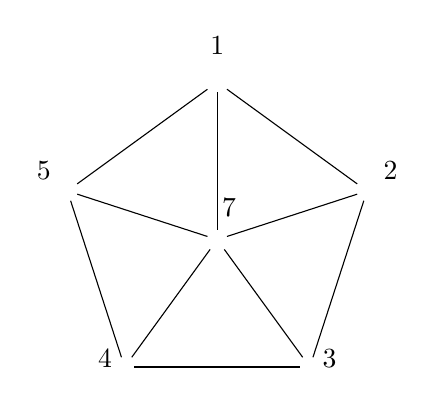
\begin{tikzpicture}
                        
\node[label={[shift={(0,0.1)}]1}](v1) at (90:2) {};

\node[label={[shift={(0.3,-0.1)}]2}](v2) at (18:2) {};

\node[label={[shift={(0.25,-0.25)}]3}](v3) at (-54:2) {};

\node[label={[shift={(-0.25,-0.25)}]4}](v4) at (234:2) {};

\node[label={[shift={(-0.3,-0.1)}]5}](v5) at (162:2) {};

\node[label={[shift={(0.15,0.05)}]7}](v7) at (0,0) {};

\foreach \from/\to in { v1/v2, v2/v3, v3/v4, v4/v5, v5/v1}
    \draw  (\from) -- (\to);
    
\foreach \from/\to in { v7/v1, v7/v2, v7/v3, v7/v4, v7/v5}
    \draw  (\from) -- (\to);


\end{tikzpicture}


\end{document} 